\chapter{Инженерная часть}

В этой главе описывается, что и как было спроектировано. При необходимости, описывается использованная методика проектирования. Сюда же относится описание внешних и внутренних программных интерфейсов, а также форматы и структуры входных и выходных данных.

%TODO Инженерная часть ...

\section{Проектирование системы геолокации по серии изображений}

\begin{figure}[h]
	\centering
	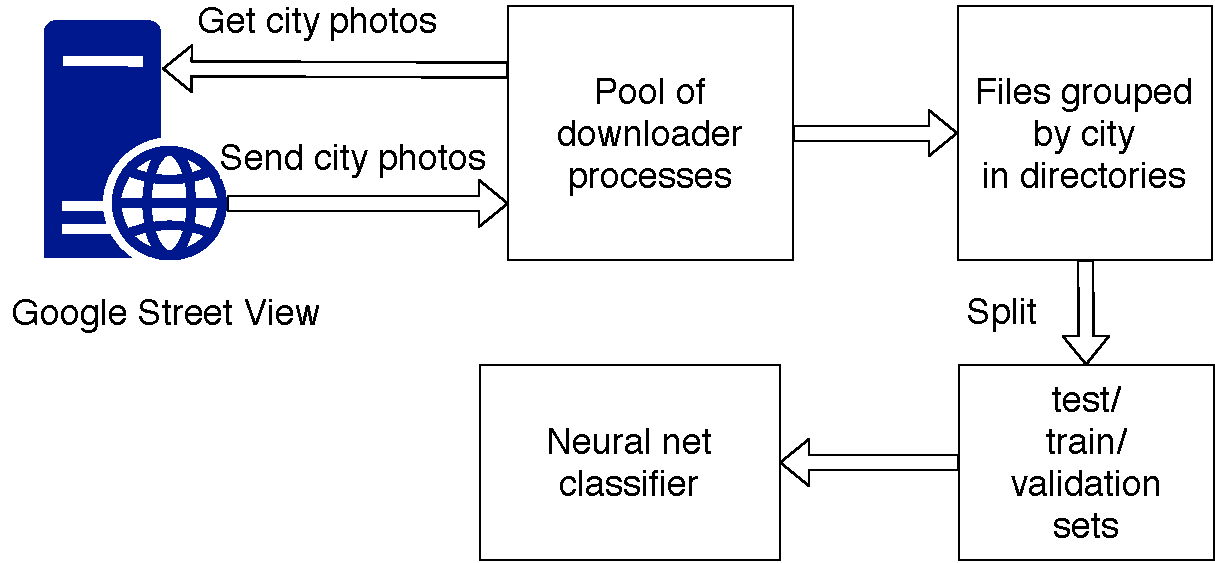
\includegraphics[width=0.7\linewidth]{img/dataset_generation}
	\caption{Схема для генерации тестового набора}
	\label{fig:datasetgeneration}
\end{figure}

Опишем на высоком уровне работу системы.

% Команда \texorpdfstring необходима, чтобы программа просмотра PDF документов
% верно отображала текст формул в панели оглавления.
% При отсутствии команды \texorpdfstring там, где она необходима, LaTeX выводит
% предупреждение "Token not allowed in a PDF string"
\section{Архитектура подсистемы генерации признаков}

\dots


\section{Архитектура подсистемы классификации}

\dots


\section{
  Проектирование протокола взаимодействия подсистем 
  классификации и генерации признаков
}

\dots


\section{Выводы}

Следует перечислить, какие инженерные результаты были получены, а именно: 
какие программные системы, подсистемы или модули были спроектированы. Следует 
не только назвать полученные архитектуры, но и отметить их отличительные 
особенности.
